\section{Analysis of structural differences}\label{sec::differences}
\subsection{Introduction}
This chapter describes the implementation of an ID-less algorithm (FMSE, described in the last chapter (\ref{subsec::ladiff})) as well as a new ID-based algorithm which utilizes a preorder traversal on both trees to compare tuples of two nodes each time. The FMSE algorithm facilitates the import of differences between two tree-structures which do not incorporate unique node-IDs in the first place either to compare different, similar tree-structures or the evolution of a tree. Thus, our similarity measures are based on the tree-to-tree correction problem. The visualizations proposed in the next chapter rely on diff-algorithms which detect edit-operations/diff-types to transform a source tree into a target tree. A reference tree is initially imported in a database system. Subsequently the changes between this tree and either other trees or the evolution of the reference-tree in terms of edit-operations are stored as subsequent revisions. As described in the last chapter, the Fast Matching Simple Edit-Script algorithm depends on similarity-measures and does not require nor use unique node-IDs in our case. Thus, a minimum edit-sequence usually is not guaranteed. While importing the differences through FMSE, the database system, Treetank assignes unique stable node-IDs which are subsequently utilized by visualizations to support a fast linear-runtime difference-computation. Fig. \ref{fig:importdata} describes the import using FMSE and a subsequent invokation of a fast ID-based diff-algorithm. When collections are going to be imported, that is multiple revisions of one tree the differences are encountered through comparing the latest stored revision in the database backend with the next revision to import. In case of multiple similar trees, the algorithm compares the first revision stored with the next revision to import. Once imported unique node-IDs and optionally hashes facilitate a new fast diff-algorithm. The computed diff-tuples which include the diff-type, the compared nodes and their depth in the tree by comparing two nodes of both revisions each time in turn facilitate an aggregated tree-structure made up of both changed- and unchanged-nodes through collecting the diff-tuples in the model of a visualization as described in the next chapter (Chapter \ref{sec::visualizations}). 

\begin{figure}[tb]
\centering
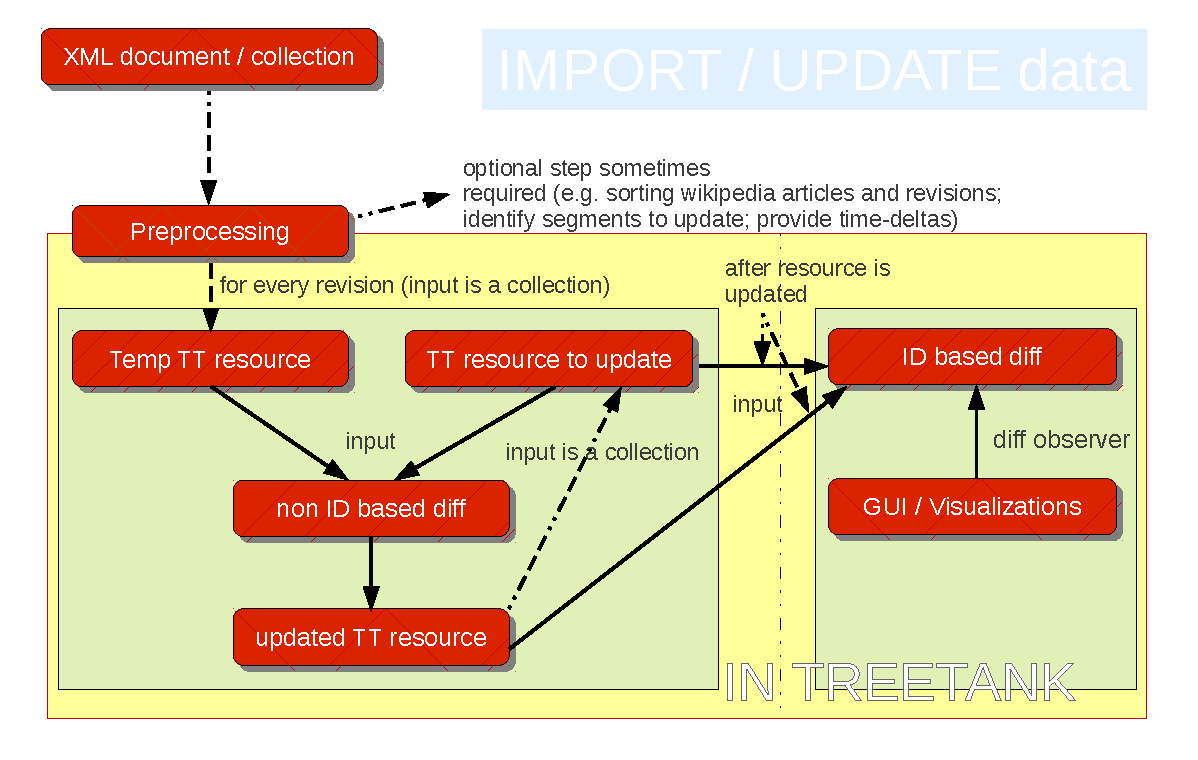
\includegraphics[width=\textwidth]{figures/importdata}
\caption{Importing differences encountered through the FMSE ID-based diffing-algorithm.} 
\label{fig:importdata}
\end{figure}

Both algorithms, the FMSE algorithm, which does not require unique node-IDs, used for importing differences and a fast ID-based diff-algorithm are implemented using Treetanks' transaction-based Java-API, the native secure tree-storage system, which is used as an integral part to demonstrate our approach. After a short description of Treetank the implementation of several new edit-operations is described to support the FMSE-algorithm and a compact, meaningful aggregated tree-structure. Note that a rich set of edit-operations also facilitates an expressive visualization. It is much more intuitive and meaningful to provide atomar \texttt{replace}- and \texttt{move}-operations to reflect changes between tree-structures than to simply use combinations of \texttt{delete}- and \texttt{insert}-operations without any association. 

%\subsection{Storage backend}
%Treetank is an effective and efficient secure storage system tailored to revisioned tree-structures. Currently it supports the import of XML documents which is commonly referred to as \emph{shredding}. To process stored data the W3C recommendations XPath 2.0, XQuery 1.0 and XSLT 2.0\footnote{parts of the XPath 2.0 recommendation have been implemented, alternatively the Saxon XPath 2.0 binding can be used which also offers the XQuery 1.0 and XSLT 2.0 support}, as well as a cursor like Java-API using transactions is supported. The architecture is based on four exchangeable vertical aligned layers. The following is a brief description of each layer in a top-down approach:

%\begin{description}
%\item[Transaction] Transactions are divided into \texttt{read}- and \texttt{write}-transactions. Read-Transactions are able to read stored nodes through a cursor-like API. Write-Transactions extend the functionality of Read-Transactions and provide both read- and write-semantics. They aditionally provide methods to modify data and commit the changes to store a new revision. Changes are atomar and saved in a transaction log which literally means they are either commited at a whole or aborted and rolled back. All ACID-properties are supported. Commiting changes results in a new appended revision, whereas nodes internally are stored based on a copy-on-write (COW) principle and a revisioning approach (full, incremental, differential and a new sliding-window\cite{kramis2009} based hybrid). Aborting a transaction means that all modifications issued during the transaction after the last commit are not persisted and lost. Update operations are applied immediately in main-memory but saved in a transaction log which is used to persist the changes after a commit. Consistency rules apply either at pre-commit time or at the time a transaction is commited.

%Every transaction includes a unique transaction ID as well as a timestamp which denotes the last commit-time of the transaction.

%\item[Node] The node layer is responsible for providing different node kinds. Currently \texttt{comment} and \texttt{processing-instruction} nodes are not supported due to the prototype research state of Treetank which is sufficient in almost all cases. Note that adding these two node types in general is straight forward. The node- and transaction-layer are responsible for the storage encoding. The main focus of the node-layer is the update-performance. Thus the pointers are stored eventuating in a local \\\texttt{key/parentKey/firstChildKey/[left|right]SiblingKey} encoding illustrated in Fig. \ref{fig:encoding}. The dashed lastChild pointer currently is not available but may be added to support efficient XPath-queries as for instance the \texttt{fn:last()}-function to get the last-element in a context-set. 

%Inserting a structural node either involves calling \texttt{insertAsFirstChild()} or \texttt{insertAsRightSibling()} on a write transaction. The first case requires to set

%\begin{itemize}
%\item the parent key to the current key located at the current transaction cursor position (before the insert)
%\item a special \texttt{NULL\_NODE\_KEY} to mark the nonexistence of any left sibling
%\item the former first child as the right sibling
%\end{itemize}

%The latter case requires to set

%\begin{itemize}
%\item the parent key to the current parent key
%\item the left sibling key to the current node key
%\item the right sibling key to the current right sibling key
%\end{itemize}

%All changes are local with a constant runtime overhead and affect at most neighbour-/parent-/child-nodes. Besides fixed length data, as the pointers to sibling/parent/firstChild nodes (which also is stored in a compressed variable length form), variable content might be stored in the node itself. For instance a hash which is used for ensuring integrity of the nodes' subtree and build through the references between the nodes is stored. In our context these hashes set the stage for an efficient ID-based diff-algorithm by comparing the hash values which is described later on in this chapter. However storing hashes (which also enables the storage of the number of descendants) at least involves updating all ancestor nodes as well depending on the specified hash-algorithm at the time generating a database.

%\begin{figure}[tb]
%\centering
%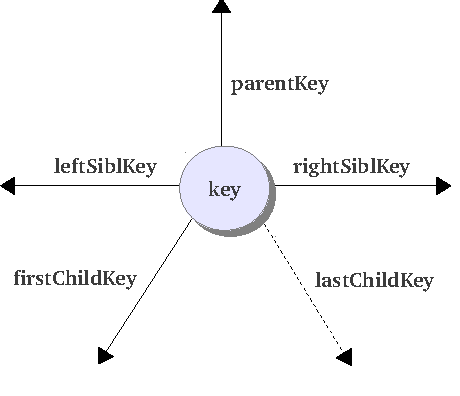
\includegraphics[width=0.45\textwidth]{figures/encoding}
%\caption{Treetank encoding} 
%\label{fig:encoding}
%\end{figure}

%\item[Page] The page-layer is motivated by ZFS \cite{ZFS}. It takes care of persisting nodes and is designed for the efficient storage of versioned tree-structures. The pages are stored in a rooted tree. A so called \emph{UberPage} contains indirect references (through references to \emph{IndirectPage}s which refer) to the stored \emph{RevisionRootPage}s. Based on the copy-on-write (COW) principle no data is lost with a minimum space consumption. Once a write transaction commits changes new \emph{NodePage}s containing modified nodes are persisted. NodePages which do not include changed nodes are not touched, therefore \emph{IndirectPage}s in subsequent revisions usually point to the same (persistent) data depending on the revisioning-strategy Treetank is configured to use.

%\item[I/O] The I/O layer is responsible for persisting and retrieving data. Currently a BerkeleyDB binding as well as a memory mapped File binding is available. A binding to Cloud Storage providers through \emph{JClouds} is in development.
%\end{description}

The next section describes the implementation of the ID-less diff algorithm called FMSE, described in general in the last Chapter (\ref{sec::relwork}).

\subsection{ID-less diff-algorithm (FMSE) / Preprocessing}
Preprocessing of raw data is a major task in every data processing pipeline. Besides data specific preprocessing, databases/resources which do not evolve through the Java-API of Treetank have to be imported. Note that it is very common to simply dump full revisions of temporal data, thus most often no direct deltas are provided which just have to be applied to a base revision. Furthermore similar distinct trees have to be compared. Both types often times do not include unique node-IDs and therefore must be compared using tree-to-tree comparison heuristics which try to determine and match the most similar nodes/subtrees. %In subsequent steps unmatched nodes are either to edit unmatched nodes afterwards (insert/delete/move). Thus, to take full advantage of the decreased storage costs regarding revisioned data in Treetank as well as to use the subsequent ID-based difference-algorithm and the visualizations, first of all differences between the tree-structures have to be computed.

%As most tree-structures do not include unique node-identifiers a diff-algorithm which compares tree-structures based on predefined similarity measures,
As described in the introduction the FMSE algorithm described in the Chapter \ref{sec::relwork} is implemented. The reasons for choosing FMSE are based on three properties: (1) it has been proven to be successfully implemented a few times (specifically for XML-documents) \cite{xmldiff}, \cite{diffxml}, (2) it utilizes a move-operation and (3) supports applying edit-operations/changes on the fly. The move-operation is one of the new edit-operation Treetank supports and very lightweight. It is defined for subtrees. Only local nodes are affected as well as the ancestor nodes of the node which moves (before and after the move). 

The Nodes are matched based on a bottom-up traversal searching for the Longest Common Subsequence (LCS) of matching nodes on each level. Predefined functions determine the similarity of nodes/subtrees as described in Chapter \ref{sec::relwork}, used by the LCS-algorithm to determine matches. Unmatched nodes after determining the LCS on each level are examined for crossmatches (moves). The algorithm not only facilitates the analysis of temporal evolving tree-structures but also the comparison of similar distinct trees. To support the FMSE implementation and expressive visualizations Treetank is enhanced in several ways. The following new operators/methods and components are available:

\begin{itemize}
\item \texttt{LevelOrderAxis} which incorporates attribute- and namespace-nodes if desired.
\item \texttt{copy-operation} to copy nodes/subtrees of other \emph{database/resource}-tuples.
\item \texttt{move-operation} to move nodes/subtrees in the currently opened \emph{resource}.
\item \texttt{replace-operation} to replace a node and its subtree with another node/subtree.
\item Visitor pattern support for nodes/transactions.
\item Merging or avoidance of adjacent text nodes.
\end{itemize}

The \texttt{LevelOrderAxis} and the other operations are described in detail in Appendix \ref{subsubsec::levelorderaxis} and \ref{subsec::operations}. Having described the preliminaries the next section describes the FMSE implementation itself.

\subsubsection{FMSE} The FMSE implementation first saves node-types and the according node-IDs in two maps during a postorder traversal. Next, the algorithm determines a longest common subsequence of matching nodes. Leaf nodes are compared first, then inner nodes. Thus the inorder-traversal described in \cite{chawathe1996change} must be replaced by a postorder-traversal. Otherwise some leaf nodes are not processed beforehand which are required to determine the similarity of inner nodes. The matching of nodes involves two different similarity-metrics as described in the last chapter. However our implementation requires some explanation, as the matching is crucial and the changes applied by FMSE are propagated to a subsequent ID-based diff-algorithm:

\begin{itemize}
\item \texttt{TextNode}s are matched based on their String-value. The Levenshtein algo\-rithm is used to compute a similarity measure of the values, which counts update costs of individual characters normalized between 0 and 1. \texttt{QName}s of \texttt{Namespace}- and \texttt{attribute}-nodes are matched first based on equality. In case of attributes afterwards their value is compared yet again using the Levenshtein algorithm in addition to their ancestor-elements.

\item \texttt{ElementNode}s are compared based on the number of matched nodes in their subtree. Recapitulate that all node-types are chained for the fast\-Matching-algorithm bottom up during a postorder traversal. Empty elements however are compared based on their \texttt{QName} similarity, whereas all ancestor nodes are also compared once more using Levenshtein. This ensures the possibility of matching empty-elements after a deletion or insertion of a subtree. Treating empty nodes as leaf nodes otherwise will prohibit matching empty \texttt{element}-nodes with other \texttt{element}-nodes which include a subtree because leaf nodes and internal nodes are compared in different successive steps and thus not cross-compared. Matching nodes are stored in a \texttt{BiMap} containing forward and backward matchings of nodeKeys.
\end{itemize}

After storing matching node-IDs, FMSE step one is implemented straight forward. However whenever an \texttt{attribute}- or \texttt{namespace}-node is determined to be moved it is deleted from the old parent and inserted at the new parent node as moves of these node-types are not permitted by Treetank. Another noteworthy subject regarding moves is, that deleted text nodes in case adjacent nodes are collapsed and must be removed from the mapping as well. Due to adding the consistency constraint that \emph{never}, before and after a commit, duplicate attributes with the same \texttt{QName} are permitted, a new attribute value is set in the \texttt{WriteTransaction.insertAttribute(QName, String)} method instead of adding a new one if the \texttt{QName} of the node to insert is identical to another attribute-node with the same parent. This also saves from time overhead due to node-creation. This case occurs whenever the attributes with the same \texttt{QName} and parent node are not matched because of very different attribute-values or parent \texttt{QName}s. All updated or inserted nodes are added to the matches as described by Chawathe et al. in \cite{chawathe1996change} to prevent them from deletion in the next step.

The second FMSE step, which deletes non matching nodes with their whole subtrees, involves a preorder traversal of the tree. Thus a new \\\texttt{VisitorDescendantAxis} which optionally expects a visitor instance is implemented \footnote{Visitors are always preferable to other methods if algorithms depend on the specific node-types, due to runtime errors during downcasts or possibly long chains of \texttt{instanceof} checks} and detailed in Appendix \ref{subsec::visitor}. 

The following cases have to be distinguished. The node to move

\begin{enumerate}
\item has no right- and no left-sibling
\item has no right- and no left-sibling but the parent has a right-sibling (the parent must be removed from a stack which is used to save right-siblings for nodes which have a first child.)
\item has a right- and a left-sibling
\item has no right- but a left-sibling
\item has a right- but no left-sibling
\end{enumerate}

Two variants of the third case are depicted in Fig. \ref{fig:deletionvisitor}. In case the node to delete has two neighbour nodes which are \texttt{TextNode}s (node 4) the right sibling node is also removed from the storage and its value is appended to the left \texttt{TextNode}. After removing the node, the transaction is located at the updated left sibling text node. Thus the preorder traversal in the \texttt{VisitorDescendantAxis} continues without skipping any nodes. Otherwise if no adjacency text nodes are merged during the remove()-operation (node 9) the transaction is moved to the right-sibling before the operation is finished. Thus, the transaction first has to be moved to the left sibling before the \texttt{VisitorDescendantAxis} moves the cursor to the right-sibling. In this case the subtree of node 8 must be skipped as it is processed before.

\begin{figure}[tb]
\center{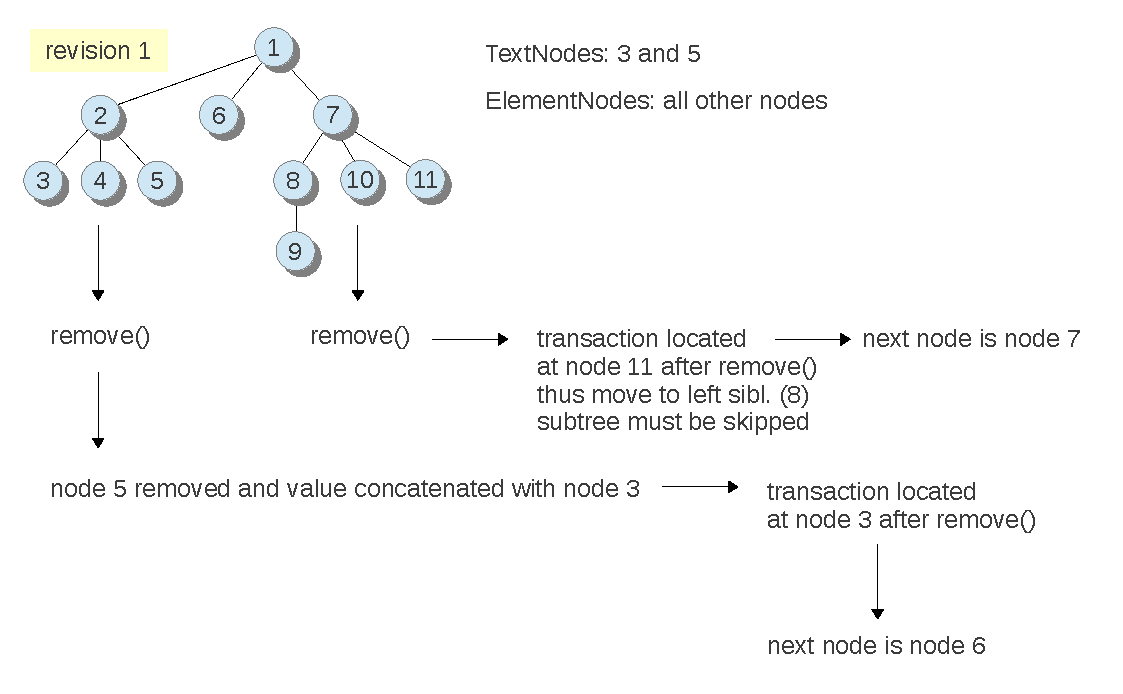
\includegraphics[width=\textwidth]
{figures/deletionvisitor}}
\caption{\label{fig:deletionvisitor} Deletion visitor; two variants are depicted if the node to removed has a left- and a right-sibling. Either both sibling nodes are \texttt{TextNode}s as is the case for node 4 or not (node 10)}
\end{figure} 

\subsection{ID-based diffing}
Once revisioned data is stored in Treetank the main task is to reveal and present structural differences of the tree-structures. Treetank supports collections in form of databases which include one or more resources. Due to stable unique node IDs in each resource every kind of tree-structure is imported updating the resource with the computed changes using FMSE. Even similar distinct tree-structures are imported updating the same resource. Otherwise, using separate resources it is not possible to utilize the unique node-IDs. Different resources do not share unique node-IDs. 

A fast diff-algorithm utilizes these unqiue node-IDs and optionally hash-values which represent the content of the entire subtree rooted at a specific node. Note that the algorithm is designed to be able to compare any two revisions and thus not just consecutive revisions. It compares two nodes each time and determines the type of diff. 

%\begin{figure}[tb]
%\center{\includegraphics[width=\textwidth]
%{figures/diff}}
%\caption{\label{fig:diff} Two revisions of a tree-structure and the edit-operations involved. By comparing consecutive revisions the edit-operations usually equal the diff-types considering \texttt{REPLACEDOLD/REPLACEDNEW} as one operation just like \texttt{MOVEDFROM/MOVEDTO}.}
%\end{figure} 

\subsubsection{Hashes} One of our goals is the efficiency of our approach as it has to be usable within interactive visualizations. Meantioned briefly in the storage section hashes of the nodes are optionally used to skip subtree-traversals if the hashes of both nodes in each revision are identical. They are build incrementally based on the nodes in the subtree bottom up either during a postorder traversal during bulk inserts or on the fly depending on the concrete hash-algorithm used. The postorder-traversal to build hashes is a new bulk-insertion method to minimize minimize affected nodes and reduce the asymptotic bound from $O(n^2)$ to $O(n)$. Two kinds of hashes are available, rolling\cite{Rolling2011}- and postorder\cite{Integrity2010}- hashes. \emph{Rolling} hashes only affect the inserted or updated nodes on the ancestor axis whereas \emph{postorder} hashes also affect nodes in a postorder traversal starting at the current node. Whenever identical hashes are determined the nodes are matched and the two transactions which compute the diff are moved to the next node in document order, which is not a descendant of the current node. Thus the transactions move to the first node in the XPath \texttt{following::}-axis. Hence, whole subtrees are skipped from traversal. The hashes include the unique node-IDs as well as node specific content. The hash-method is designed to be fast and to reduce collisions to a minimum. Even if hash-collisions which are extremely unlikely appear it is not possible to match subtrees with same hash-values as the node-IDs are also compared which are stable and unique during all revisions. Rolling-hashes are enabled by default during the database/resource creation and optionally used by our diff-algorithm. It is for instance used by an optional pruning of the tree in a Sunburst-layout to speed up the computation as well as the construction of the visualization. An in depth explanation of this application is provided in the Chapter \ref{sec::visualizations}. The next subsection briefly described two modes of the algorithm.

\subsubsection{Kind of differences} Interested observers are notified of the diff between two nodes through registration and the implementation of a special interface method. Currently two kinds of diffs are available.

\begin{itemize}
\item \emph{Structural Diff} calculates changes without comparing attribute and namespace nodes. This implies that whenever the overall structure is crucial this algorithm should be chosen.
\item \emph{Full Diff} takes structural nodes as well as attribute and namespace nodes into account. However currently we do not emit non-structural changes. Changes in \texttt{namespace}- or \texttt{attribute}-nodes results in an \texttt{UPDATED} parent-element. This restriction applies as the \emph{SunburstView} which is described in Chapter \ref{sec::visualizations} currently does not include special \texttt{namespace}- or \texttt{attribute}-items. Instead these are part of the element item and shown on mouseover.
\end{itemize}
They are implemented by a simple template method\\ \texttt{checkNode(IReadTransaction, IReadTransaction)} which is called by the basic diff-algorithm.

The following diff-types are supported by the algorithm:

\begin{itemize}
\item \texttt{INSERTED} denotes that a node is inserted.
\item \texttt{DELETED} denotes that a node is removed.
\item \texttt{UPDATED} denotes that a node is updated, that is either the QName of an \texttt{element}-node is updated or the value of a \texttt{text}-node.
\item \texttt{SAME} denotes that a node is not changed.
\item \texttt{REPLACEDOLD} denotes that a node or subtree is replaced (the old node/subtree).
\item \texttt{REPLACEDNEW} denotes that a node or subtree is replaced (the new node/subtree).
\item \texttt{SAMEHASH} denotes that a node is not changed and the hashes of the subtrees are identical.
\end{itemize}

Note that the differentiation between \texttt{REPLACEDOLD/REPLACEDNEW} is to support an expressive aggregated tree-structure as an underlying model of the visualizations. Two other diff-types are supported by an optional post-processing step.

\begin{itemize}
\item \texttt{MOVEDFROM} denotes that a node or whole subtree has been moved from this location to another one.
\item \texttt{MOVEDTO} denotes that a node or whole subtree has been moved to this location.
\end{itemize}

The types are splitted, too to indicate the movemenet of the node, the old place as well as the new place in the aggregated tree-structure.

\subsection{Traversal of both revisions}
The algorithm to traverse the trees and to compute the differences between two nodes in each revision is depicted in algorithm \ref{overallDiffAlgo}. First, the method\\ \texttt{treeDeletedOrInserted(IReadTransaction, IReadTransaction)} checks if\\ both transactions opened on each revision can be moved to the start node. If not, either the node is inserted or deleted depending on the transaction which can not be moved.

Let's examine both cases:
\begin{itemize}
\item
The transaction opened on the older revision can not be moved to the start node. This implies that the tree in the new revision has been inserted.
\item
The transaction opened on the newer revision can not be moved to the start node. This implies that all nodes in the old transaction have been deleted.
\end{itemize}

The distinction is used to support the selection of modified nodes in the visualizations which are described in Chapter \ref{sec::visualizations} and only affects subtrees. Otherwise simply put all nodes in the old revision must be deleted, whereas all nodes in the new revision are inserted.

If the root-nodes of both revisions are selected by the transactions they move forward in \emph{document order} (depicted in Fig. \ref{fig:id-diff}) depending on the last encountered kind of diff between two nodes. Document order is identical to a preorder traversal of a tree. In case of an insert, the transaction opened on the new revision is moved forward, in case of a delete the transaction opened on the old revision is moved (the \\ \texttt{moveCursor(IReadTransaction, ERevision)}-method). If a node is updated or has not been changed at all both transactions move to the next node in document order. Once the traversal in one of the two revisions is done, the transaction is located at the document root. The diff-calculation ends if either the transaction on the older revision is located at the document root and the last encountered diff kind was \texttt{DELETED} or both transactions are located at the document-root of both revisions. Note that if the transaction on the newer revision is located at the document root, but the transaction on the old revision is not the following nodes are \texttt{DELETED} at the end of the tree and have to be emitted as such (lines 22-28). 

\begin{figure}[tb]
\center{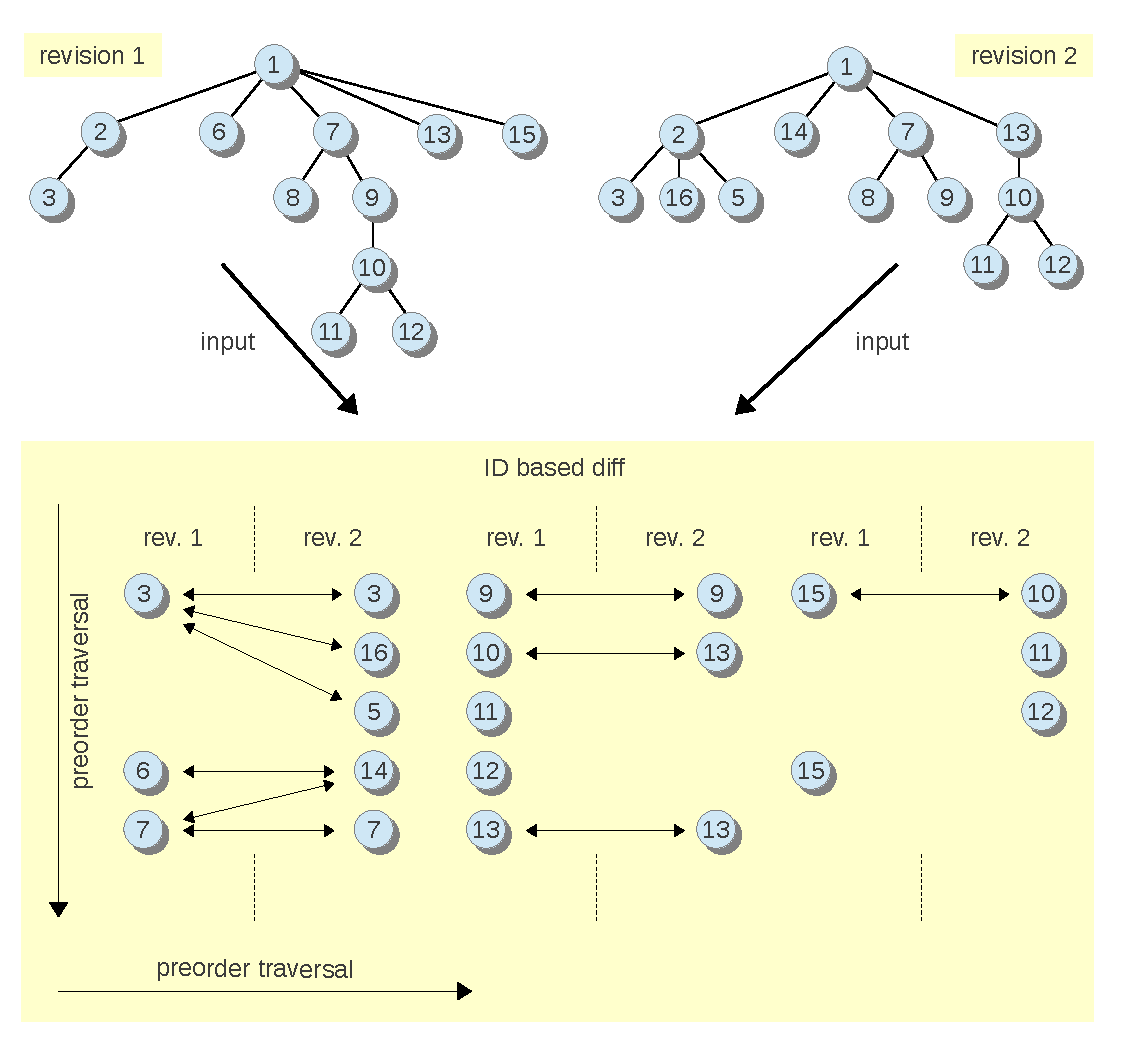
\includegraphics[width=\textwidth]
{figures/id-diff}}
\caption{\label{fig:id-diff} ID-based diffing.}
\end{figure} 

\begin{algorithm}[Hhtbp]
\SetKwInOut{Input}{input}\SetKwInOut{Output}{output}
\Input{HashKind mHashKind, long pOldRevKey, long pNewRevKey, long mOldStartKey, long mNewStartKey, DiffType pDiffType, DiffTypeOptimized mDiffKind, ISession mSession}
\Output{for each node comparsion: DiffType diffType, IStructNode oldNode, IStructNode newNode, Depth depth}
\BlankLine
INodeReadTransaction rtxOld $\leftarrow$ mSession.beginNodeReadTransaction(pOldRevKey)\;
INodeReadTransaction rtxNew $\leftarrow$ mSession.beginNodeReadTransaction(pNewRevKey)\;
\tcp{moveTo(long) returns true in case the transaction could be moved to the node or false otherwise.}
newRtxMoved $\leftarrow$ rtxNew.moveTo(mNewStartKey)\;
oldRtxMoved $\leftarrow$ rtxOld.moveTo(mOldStartKey)\;

treeDeletedOrInserted(newRtxMoved, oldRtxMoved)\;

DiffType $\leftarrow$ null\;
\tcp{Check first node.}
\If{mHashKind == HashKind.None OR mDiffKind == DiffTypeOptimized.NO}{
  diff $\leftarrow$ diff(rtxNew, rtxOld, depth)\;
}\Else{
  diff $\leftarrow$ optimizedDiff(rtxNew, rtxOld, depth)\;
}

\tcp{Iterate over new revision (order of operators significant -- regarding the OR).}
\If{diff != DiffType.SAMEHASH}{
  \While{(rtxOld.getNode().getKind() != ENode.ROOT\_KIND AND diff == DiffType.DELETED) OR moveCursor(rtxNew, ERevision.NEW)}{
  \If{diff != DiffType.INSERTED}{
    moveCursor(rtxOld, ERevision.OLD)\;
  }

  \If{rtxNew.getNode().getKind() != ENode.ROOT\_KIND
   or rtxOld.getNode().getKind() != ENode.ROOT\_KIND}{
    \If{mHashKind == HashKind.None OR mDiffKind == DiffTypeOptimized.NO}{
      diff $\leftarrow$ diff(rtxNew, rtxOld, depth)\;
    }\Else{
      diff $\leftarrow$ optimizedDiff(rtxNew, rtxOld, depth)\;
    }
  }
}

\tcp{Nodes deleted in old rev at the end of the tree.}
\If{rtxOld.getNode().getKind() != ENode.ROOT\_KIND}{
  emitOldNodes(rtxNew, rtxOld, depth)\;
}
}

done()\;
\caption{ID-based diff: traversal}\label{overallDiffAlgo}
\end{algorithm}

\subsection{Diff-Computation}
Besides moving both transactions forward in document-order depending on the type of diff the computation which determines the diff-type itself is crucial. The computation is the main task of the \\ \texttt{diff(INodeReadTransaction, INodeReadTransaction, Depth)}-method outlined in algorithm \ref{diffAlgo}. It is invoked whenever the node-IDs or the \texttt{QName}s/\texttt{Text}-values of the nodes to compare differ.

\begin{algorithm}[Hhtbp]
\SetKwInOut{Input}{input}\SetKwInOut{Output}{output}
\Input{Depth pDepth, INodeReadTrx pOldRtx, INodeReadTrx pNewRtx}
\Output{kind of diff (DiffType enum value)}
\BlankLine
DiffType diff $\leftarrow$ DiffType.SAME;

\tcp{Check if node has been deleted.}
\If{pDepth.getOldDepth() $>$ pDepth.getNewDepth())}{ 
  diff $\leftarrow$ DiffType.DELETED\;
  cumulatDiffTypes(diff)\;
  \If{checkReplace(pNewRtx, pOldRtx)}{
        diff $\leftarrow$ DiffType.REPLACED\;
  }
}\tcp{Check if node has been updated.}\ElseIf{checkUpdate(pNewRtx, pOldRtx)}{ 
  diff $\leftarrow$ DiffType.UPDATED\;
}\tcp{Check if node has been replaced.}\ElseIf{checkReplace(pNewRtx, pOldRtx)}{ 
  diff $\leftarrow$ DiffType.REPLACED\;
}\Else{
  long oldKey $\leftarrow$ pOldRtx.getNode().getNodeKey()\;
  boolean movedOld $\leftarrow$ pOldRtx.moveTo(pNewRtx.getNode().getNodeKey())\;
  pOldRtx.moveTo(oldKey);

  long newKey $\leftarrow$ pNewRtx.getNode().getNodeKey()\;
  boolean movedNew $\leftarrow$ pNewRtx.moveTo(pOldRtx.getNode().getNodeKey())\;
  pNewRtx.moveTo(newKey);

  \If{!movedOld}{
    diff $\leftarrow$ DiffType.INSERTED\;
  }\ElseIf{!movedNew}{
    diff $\leftarrow$ DiffType.DELETED\;
  }\Else{
    \tcp{Determine if one of the right sibling matches.}
    EFoundEqualNode found $\leftarrow$ EFoundEqualNode.FALSE\;
    long key $\leftarrow$ pOldRtx.getNode().getNodeKey()\;

    \While{pOldRtx.getStructuralNode().hasRightSibling() AND pOldRtx.moveToRightSibling()
      AND found == EFoundEqualNode.FALSE}{
      \If{checkNodes(pNewRtx, pOldRtx)}{
        found $\leftarrow$ EFoundEqualNode.TRUE\;
        break\;
      }
    }

    pOldRtx.moveTo(key)\;
    diff $\leftarrow$ found.kindOfDiff()\;
  }

  cumulatDiffTypes(diff)\;
}

return diff\;
\caption{ID-based diff: diff-computation}\label{diffAlgo}
\end{algorithm}

First, the depths of the nodes have to be compared. The depth is the sum of nodes in the path up to the root-node. When the depth of the node in the old revision is greater than the depth of the node in the new revision it must have been deleted. Note that the depths are not persisted, thus counters have to keep track of the current depths. All diff-tuples which are of type \texttt{DiffType.DELETED} or \texttt{DiffType.INSERTED} are saved in a Java \texttt{List}. A second datastructure is used to gather the diff types itself, that is a whole subtree which is either inserted or deleted is cumulated by the according diff-type. This datastructure is used to find \texttt{INSERTED}, \texttt{DELETED} combinations which are instead emitted as of type \texttt{DiffType.REPLACEDOLD} (the deleted tuples) and \texttt{DiffType.REPLACENEW} (the inserted tuples).

When the depth of the node in the old- and the node in the new-revision instead either is identical or the depth of the node in the more recent revision is greater at first the node is checked for an update through comparison of the nodeKeys and the depths of the nodes. Unless the check yields true the nodes are examined for replacement. Therefore the datastructure which keeps track of deleted- and inserted-subtrees is reviewed. Consecutive insert/delete- or insert/insert/delete/delete-tuples are emitted as replaced subtrees. Note that this replace-detection is just a simple heuristic and currently does only detect the aforemeantioned pairs of inserted and deleted nodes.%The datastructure in either case is emptied even if no matching types are found. Furthermore when two diff-types previously have been stored in the datastructure the \texttt{List} of diff-tuples must immediately be emitted in case a replace has been detected and the datastructure must be reinitialized \footnote{for instance replaced with a new instance} afterwards. Four elements are always immediately emitted regardless of whether the diff-types have changed or not. In the first case subsequently the replaced tuples must be emitted.

Assuming a node or subtree is not replaced, it must be decided if either the current node in the new revision is inserted or the current node in the old revision is deleted. First, it is determined if the transaction opened on the old revision is moveable to the current node in the new revision. If not it is immediately obvious that the node is inserted. Otherwise, if the transaction opended on the new revision can \emph{not} be moved to the current node in the old revision it must be a deleted node. For the simple reason that move-operations are supported both checks might succeed. In this case the right siblings of the node in the old revision have to be examined in order to determine the type of diff, until one of them matches the node in the new revision, that is the node-IDs are identical or no more right siblings are available. In the first case the new node is inserted. Otherwise it is deleted.

\subsection{Detecting moves}
An optional postprocessing step is required to detect moves. The two basic diff-types \texttt{MOVEDFROM} and \texttt{MOVEDTO} are detected after all operations are emitted. The detection requires three datastructures to store all diff-types, the inserted nodes and the deleted nodes.

\subsubsection{Impossible to detect moves on the fly} Note that it is not possible to include the detection of moves in the preorder-traversal of both revisions itself, as it is not known which of the two nodes is the one which has been moved and which one is the node which is unchanged. However this is required to determine which of the two transactions must be moved to the next node in document order. All we can argue is, that it would be possible to detect a move itself if the transaction on the new revision can be moved to the current node from the transaction in the old revision and vice versa. That is all \texttt{DELETED} or \texttt{INSERTED} nodes have already been emitted, meaning that one of the two nodes which are currently compared must have been moved and the other must have been unchanged constant. It is not possible to decide which one of the two nodes stayed the same and which one has been moved. The position in the tree is no implication wheter a node has been moved from or moved to another place, but this is crucial to decide which of the two nodes has not changed and which one actually has been moved. As thus the types have to be matched. Whenever the unique nodeKey of a \texttt{DELETED}-node matches the key of an \texttt{INSERTED}-node, the corresponding diff-types can be changed into \texttt{MOVEDFROM} and \texttt{MOVEDTO}. The next subsection details a postprocessing algorithm which is based on this idea.

\subsubsection{Detection of moves in a postprocessing step} All encountered diff-types are saved in an associative array, a map (index of their encounter $\Leftrightarrow$ diff-tuple) \footnote{which is used just like a List, to switch between a map implementation based on a persistent  BerkeleyDB database depending on a specified threshold value or a simple LinkedHashMap instance} in preorder which is the order in which they have been observed. Additionally \texttt{DELETED} and \texttt{INSERTED} nodes are recorded mapping their unique nodeKey to the index in the original map with all entries. The algorithm described in \ref{diffPostprocessing} expects the three maps. It tries to match \texttt{INSERTED} $\Leftrightarrow$ \texttt{DELETED} pairs and vice versa and checks whether the diffType in the map needs to be adjusted to \texttt{MOVEDTO} or \texttt{MOVEDFROM} (or not at all). A map which does not contain a value for the specified key returns the special value \texttt{null}. First, the old nodeKey (might have been deleted) is searched for in the Map containing all inserted tuples. If the key is found (value $!=$ null) the type is checked. If the current diff-tuple is of type \texttt{DELETED} or \texttt{MOVEDFROM} the diff type is set to \texttt{MOVEDTO}. Note that the check for the \texttt{MOVEDFROM} type is necessary as the corresponding \texttt{INSERT} tuple might have been encountered before and thus the type has been changed to \texttt{MOVEDFROM} already. The following is the inverse case to set the \texttt{MOVEDFROM} type if necessary. Furthermore a link in the form of the index of the matching node with the same nodeKey and the corresponding \texttt{MOVEDTO} diff-type is additionaly saved. Note that the algorithm does not detect \texttt{text}-nodes which are moved to a right sibling of another \texttt{text}-node. In this case our implementation of the \texttt{moveSubtreeToRightSibling(long)} prepends the value of the current \texttt{text}-node to the moved \texttt{text}-node and subsequently deletes the current node. This ensures, that no two text-nodes are ever adjacent which otherwise contradicts the XQuery/XPath data model (XDM). In this particular edge case the algorithm determines a \texttt{REPLACED} node (a direct consequent from the deletion of the node the transaction resides at and the insertion of the moved node with the prepended text-value) and a \texttt{DELETED} node (the node which has been moved).

\begin{algorithm}[Hhtbp]
\SetKwInOut{Input}{input}\SetKwInOut{Output}{output}
\Input{Map allDiffs, Map inserted, Map deleted}
\Output{none (void)}
\BlankLine
\tcp{For every diff tuple in the map which saves all encountered diffs in document-order}
\For{Diff diffTuple : allDiffs.values()}{
  Integer newIndex $\leftarrow$ inserted.get(diffTuple.getOldNodeKey())\;
  \If{newIndex != null
    AND (diffTuple.getDiff() == DiffType.DELETED OR diffTuple.getDiff() == DiffType.MOVEDFROM)}{
      allDiffs.get(newIndex).setDiff(DiffType.MOVEDTO)\;
  }
  Integer oldIndex $\leftarrow$ deleted.get(diffCont.getNewNodeKey())\;
  \If{oldIndex != null
    AND (diffTuple.getDiff() == DiffType.INSERTED OR diffTuple.getDiff() == DiffType.MOVEDPASTE)}{
      allDiffs.get(oldIndex).setDiff(DiffType.MOVEDFROM).setIndex(
                 inserted.get(diffTuple.getNewNodeKey()))\;
  }
}
\caption{ID-based diff: postprocessing to detect moves}\label{diffPostprocessing}
\end{algorithm}

\subsection{Runtime/Space analysis and scalability of the ID-based diffing algorithm}
The runtime of the ID-based diff algorithm is $O(n+m)$ whereas $n$ is the number of nodes in the first tree and $m$ the number of nodes in the second tree. It is thus a fast linear diff-computation in comparison to the FMSE-algorithm ($O()$) which is used in the first place to determine the differences which are imported. The space-consumption is $O(1)$ and in case the replace-operation is enabled at worst $O(k)$ whereas k is the sum of the subtrees which are cached (at most 4 subtrees currently). However the space consumption of an aggregated tree-structure which is going to be described in the next chapter (\ref{sec::visualizations}) is $O(u*k+v*k)$. $u$ is the number of unchanged nodes, $v$ is the number of changed nodes and $k$ is tuple relevant stuff (type of diff, the nodes and the depths in both trees). Thus the asymptotic space consumption is linear depending only on the number of unchanged and changed nodes.

Our performance evaluation involves measuring the scaling during random modification-patterns (Fig. \ref{fig:100MBscaling}) and different document sizes with scaled modification-patterns (Fig. \ref{fig:docScaling}). The modification-patterns are increased in the same scale as the document size such that the documents are modified with approximately the same number of modifications. The hardware used is a common notebook with 4Gb RAM and a Core 2 Duo 2,66 Ghz CPU. All performance-measures are executed 20 times. Fig. \ref{fig:100MBscaling} shows that the number of modifications minimally affects the runtime. The runtime decreases linear as less modifications between two revisions are encountered. However the linear decrease is minimal due to a few more value and node-ID comparisons.

\begin{figure}[tb]
\centering
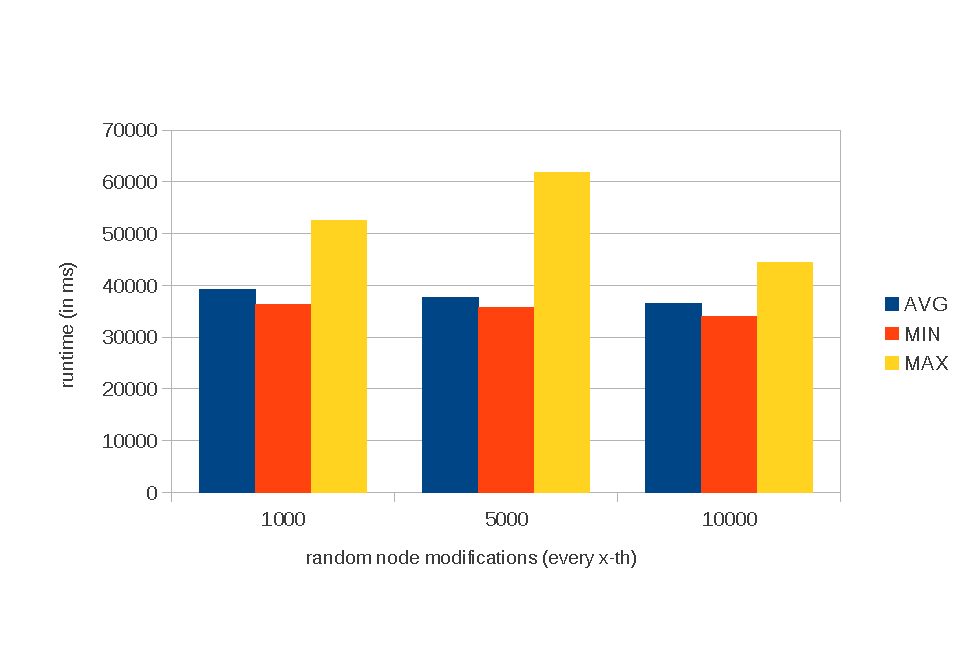
\includegraphics[width=\textwidth]{figures/100MB-scaling}
\caption{Scaling during different modification-patterns (update/insert/delete/replace/move every 1000st, 5000st and 10000st node) in a 111 MiB XMark instance.} 
\label{fig:100MBscaling}
\end{figure}

\begin{table}[tb]
\centering 
\begin{tabular}[r]{|l|c|c|c|} 
\hline
& \textbf{1000mods} & \textbf{5000mods} & \textbf{10000mods}\\
\hline
\hline
\textbf{min} & 36265.14 & 35717.34 & 33948.96\\
\hline
\textbf{max} & 52459.38 & 61860.29 & 44451.06\\
\hline
\textbf{average} & 39167.75 & 37650.67 & 36579.37\\
\hline
\end{tabular}
\label{chap3:comparsion}
\vspace{0.5em} 
\caption{Comparsion of different modification-patterns of a 111 MiB XMark instance (update/insert/delete/replace/move every 1000st, 5000st and 10000st node). Runtime in ms.}
\end{table}

Fig. \ref{fig:docScaling} (Table \ref{chap3:compDiffInstances}) depicts the scaling during different document sizes and modification schemes. The scale is logarithmic, thus we are able to identify the linear runtime due to increased document sizes. It therefore emphasizes the asymptotic bound.

\begin{figure}[tb]
\centering
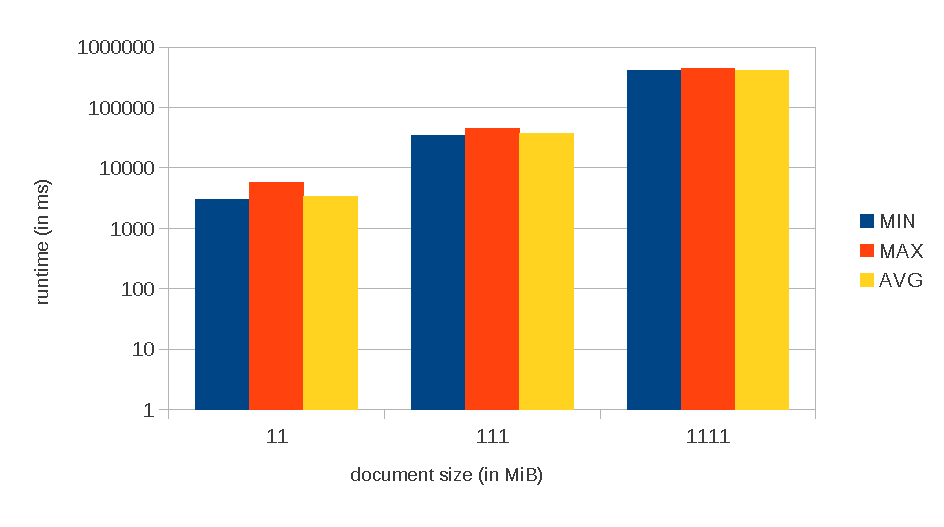
\includegraphics[width=\textwidth]{figures/diff-docsize-scale}
\caption{Different document sizes with modification-count scaled accordingly (11 MiB $\Leftrightarrow$ modifiy every 1000th node, 111 MiB $\Leftrightarrow$ modify every 11000 th node, 1111 MiB $\Leftrightarrow$ modify every 122221th node / Y-axis logarithmic scaled)} 
\label{fig:docScaling}
\end{figure}

\begin{table}[tb]
\centering 
\begin{tabular}[r]{|l|c|c|c|} 
\hline
& \textbf{11 MiB} & \textbf{111 MiB} & \textbf{1111 MiB}\\
\hline
\hline
\textbf{min} & 2957.79 & 33948.96 & 401878.64\\
\hline
\textbf{max} & 5694.65 & 44451.06 & 439337.71\\
\hline
\textbf{average} & 3323.96 & 36579.37 & 413158.13\\
\hline
\end{tabular}
\label{chap3:compDiffInstances}
\vspace{0.5em} 
\caption{Comparsion of different XMark instances (11 MiB, 111 MiB, 1111 MiB modifying every 1000st, 11000st and 122221st node). Runtime in ms.}
\end{table}

Table \ref{chap3:compPrunedDiffInstances} shows the comparison based on the same documents as in Table \ref{chap3:compDiffInstances} however this time utilizing the hashes to skip the traversal of unchanged subtrees (nodes with identical hash-values and node-IDs). The runtime approximately halves in this example. It is obvious that the gain in speed depends on the subtree-sizes to skip. The worst case are modifications at leaf nodes in large, deep subtrees. In this case the hash-based optimization does not gain any speedup (in the 11 MiB XMark document with all leaf nodes updated approximately 4062.52ms in the average case compared to 4064.96ms for the hash-based optimization after 20 runs). The best case is to have modifications near the root node of large, deep subtrees (in the 11 MiB XMark document with depth 2 updated the runtime drops from 31979.92ms to 12280.01ms in the averge case). However, the XMark synthetic documents are not very deep, such that usually only a few nodes are skipped for every identical hash-value.

\begin{figure}[tb]
\centering
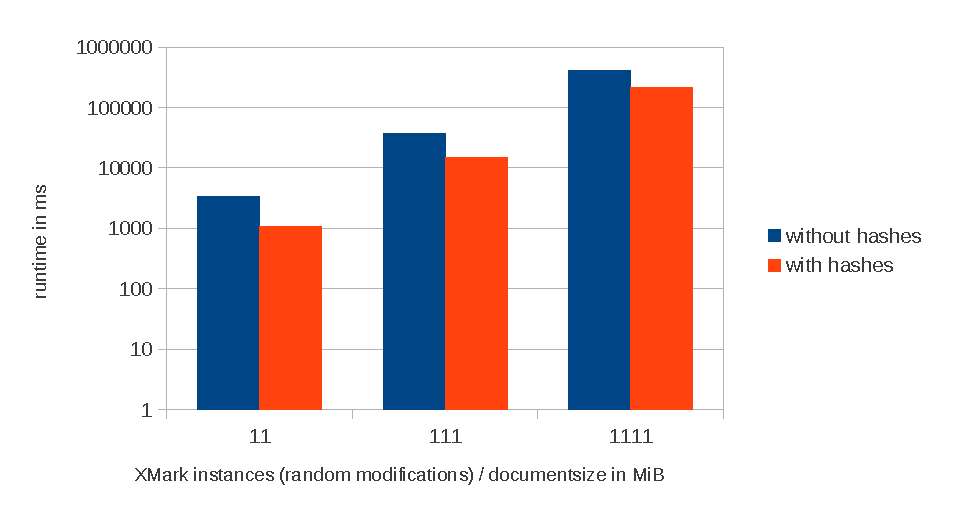
\includegraphics[width=\textwidth]{figures/diff-docsize-scale-pruned}
\caption{Different document sizes with modification-count scaled accordingly (11 MiB $\Leftrightarrow$ modifiy every 1000th node, 111 MiB $\Leftrightarrow$ modify every 11000 th node, 1111 MiB $\Leftrightarrow$ modify every 122221th node / Y-axis logarithmic scaled)} 
\label{fig:docScaling}
\end{figure}

\begin{table}[tb]
\centering 
\begin{tabular}[r]{|l|c|c|c|} 
\hline
& \textbf{11 MiB} & \textbf{111 MiB} & \textbf{1111 MiB}\\
\hline
\hline
\textbf{min} & 1239.01 & 14208.30 & 197223.12\\
\hline
\textbf{max} & 3698.94 & 19135.01 & 271794.82\\
\hline
\textbf{average} & 1408.74 & 14596.86 & 210296.70\\
\hline
\end{tabular}
\label{chap3:compPrunedDiffInstances}
\vspace{0.5em} 
\caption{Comparsion of different XMark instances skipping subtrees of nodes with identical hash-values (11 MiB, 111 MiB, 1111 MiB modifying every 1000st, 11000st and 111000st node). Runtime in ms.}
\end{table}

\subsection{Conclusion and Summary}
We motivated the import of differences between full dumps of temporal tree-structures to subsequently take full advantage of Treetanks' (1) revisioning strategies, (2) unique node-IDs which identify a node through all revisions and (3) hashes of each node, which almost guarantee a unique hash guarding the whole subtree through cryptographic rolling hashes. The FMSE-algorithm is implemented to support the initial import of differences in these full dumps, that is revisioned data (currently) in the form of XML-documents whereas each document represents one revision, a snapshot at a specific time. Considering no such data is available other even more sophisticated preprocessing steps have to be implemented and executed before a diff-algorithm on the revisioned data in Treetank is useable. Two of the use cases which are going to be discussed in Chapter \ref{sec::applications} require further preprocessing. Note that the FMSE-algorithm is used to import data which does not assume unique node-IDs and matches nodes based on a longest common subsequence (LCSS)-calculation (which is ambiguous) for leaf nodes and inner nodes in a bottom up traversal. Thus it might mismatch similar nodes eventuating in too many edit-operations. The algorithm is particularly useful to compare similar different tree-structures which do not temporally evolve and usually naturally do not include node-IDs.

Furthermore we have implemented many edit-operations which were not available in Treetank to support the implementation of the FMSE-algorithm and a very expressive agglomerated tree-structure. We have shown that a subsequent diff-calculation based on IDs and hashes which guard the whole subtree is faster than the same algorithm without utilizing hashes. However it depends on the properties of the tree-structures. If large subtrees can be skipped due to same hashes meaning they are unchanged the running time is reduced drastically.

Besides using hashes optionally to skip whole unchanged subtrees our ID-based diff-algorithm combines \texttt{INSERT/DELETE} and \texttt{DELETE/INSERT} sequences to a single replace-operation. To support an agglomerated tree-structure which incorporates nodes of both compared revisions described in the next chapter either emits diff-tuples of type \texttt{REPLACEDOLD} or \texttt{REPLACEDNEW} depending on which of the two subtrees are larger, thus increasing the expressiveness. Note that this detection potentially involves a lot of state if large subtrees are inserted/deleted or vice versa successively. Therefore we additionally provide a different replace-detection which uses heuristics checking right-sibling nodeKeys for equivalence or the parent node keys if in both revisions no right sibling exists).

Moves are optionally detected in a postprocessing-step by searching for \\\texttt{INSERT/DELETE} and \texttt{DELETE/INSERT} combinations with the same node-IDs. Move detection is especially useful to support analysts with an expressive visualization. Otherwise in document-centric XML, for instance DocBook\cite{docbook} documents, it might be impossible to draw conclusions from simple inserts/deletes, whereas an author simply moved a sentence along with other inserts/deletions of text and/or markup.
